\newcommand*{\examnumber}{B135653}
\newcommand*{\field}{Resiliant supply chains in OpenTTD}
\newcommand*{\tutor}{Bob Fisher}
\newcommand*{\supervisor}{Michael Herrmann}
\newcommand*{\KEYWORDS}{\field, \supervisor, \tutor, School of Informatics, University of Edinburgh}

%
%                       This is a basic LaTeX Template
%                       for the Informatics Research Review

\documentclass[a4paper,11pt]{article}
% Add local fullpage and head macros
\usepackage{head,fullpage}     
% Add graphicx package with pdf flag (must use pdflatex)
\usepackage[pdftex]{graphicx}  
% Better support for URLs
\usepackage{url}
% Date formating
\usepackage{datetime}
% For Gantt chart
\usepackage{pgfgantt}
\usepackage{xcolor}
\usepackage[utf8]{inputenc}

\definecolor{hyperlinkColor}{HTML}{0D3B68}
\usepackage[shrink=20,stretch=20]{microtype}
\usepackage{siunitx}
\sisetup{detect-all
  ,group-minimum-digits=3% Western convention is groups of 3 digits
  ,mode = text
%   ,text-font-command = \liningroman
}
\usepackage{xurl}
\usepackage{hyperref}
\hypersetup{%
   pdfauthor=\texorpdfstring{\examnumber}{\examnumber}%
  ,pdftitle=\texorpdfstring{\field}{\field}%
  ,pdfsubject=\texorpdfstring{\field}{\field}%
  ,pdfkeywords=\texorpdfstring{\KEYWORDS}{\KEYWORDS}%
  ,linktoc=all%
  ,colorlinks=true%\ifdefstring{\expandafter\docUsage}{print}{false}{true}
  ,linkcolor=hyperlinkColor
  ,linkbordercolor=hyperlinkColor% internal hyperlink border colour
  ,urlcolor=hyperlinkColor
  ,urlbordercolor=hyperlinkColor% external hyperlink border colour
  ,citecolor=hyperlinkColor
  ,citebordercolor=hyperlinkColor% internal citation border colour
  ,pdfborderstyle={/S/U/W 1.5}% border style will be an underline of width 1.5pt
}

\usepackage{cleveref}
\usepackage[shortcuts]{extdash}
% gives \=/ for non-breaking hyphen
% and \-/ to allow the word before the hyphen to be hyphenated
\newdateformat{monthyeardate}{%
  \monthname[\THEMONTH] \THEYEAR}

\parindent=0pt          %  Switch off indent of paragraphs 
\parskip=5pt            %  Put 5pt between each paragraph  
\Urlmuskip=0mu plus 1mu %  Better line breaks for URLs


%                       This section generates a title page
%                       Edit only the following three lines
%                       providing your exam number, 
%                       the general field of study you are considering
%                       for your review, and name of IRR tutor
\usepackage{floatpag}
\floatpagestyle{empty}

\begin{document}
\begin{minipage}[b]{110mm}
        {\Huge\bf School of Informatics
        \vspace*{17mm}}
\end{minipage}
\hfill
\begin{minipage}[t]{40mm}               
        \makebox[40mm]{
        
\includegraphics[width=40mm]{crest.png}}
\end{minipage}
\par\noindent
    % Centre Title, and name
\vspace*{2cm}
\begin{center}
        \Large\bf Informatics Project Proposal \\
        \Large\bf \field
\end{center}
\vspace*{1.5cm}
\begin{center}
        \bf \examnumber\\
        \monthyeardate\today
\end{center}
\vspace*{5mm}

%
%                       Insert your abstract HERE
%                       
\begin{abstract}
OpenTTD \cite{openttd} is an open source supply chain simulation computer game based on the 1990s game Transport Tycoon Deluxe. OpenTTD allows the creation of so-called AIs: computer players that build supply chains to compete with human players. This project is to create such an AI that builds supply chains with good resilience properties. The focus of this project is the game, but it will add to the body of research into real-world supply chains affected by the coronavirus (COVID-19) pandemic.
\end{abstract}

\vspace*{1cm}

\vspace*{3cm}
Date: \today

\vfill
{\bf Tutor:} \tutor\\
{\bf Supervisor:} \supervisor
\newpage

%                                               Through page and setup 
%                                               fancy headings
\setcounter{page}{1}                            % Set page number to 1
\footruleheight{1pt}
\headruleheight{1pt}
\lfoot{\small School of Informatics}
\lhead{Informatics Research Review}
\rhead{- \thepage}
\cfoot{}
\rfoot{Date: \date{\today}}
%


\section{Motivation}

\begin{figure}[h]
\centering
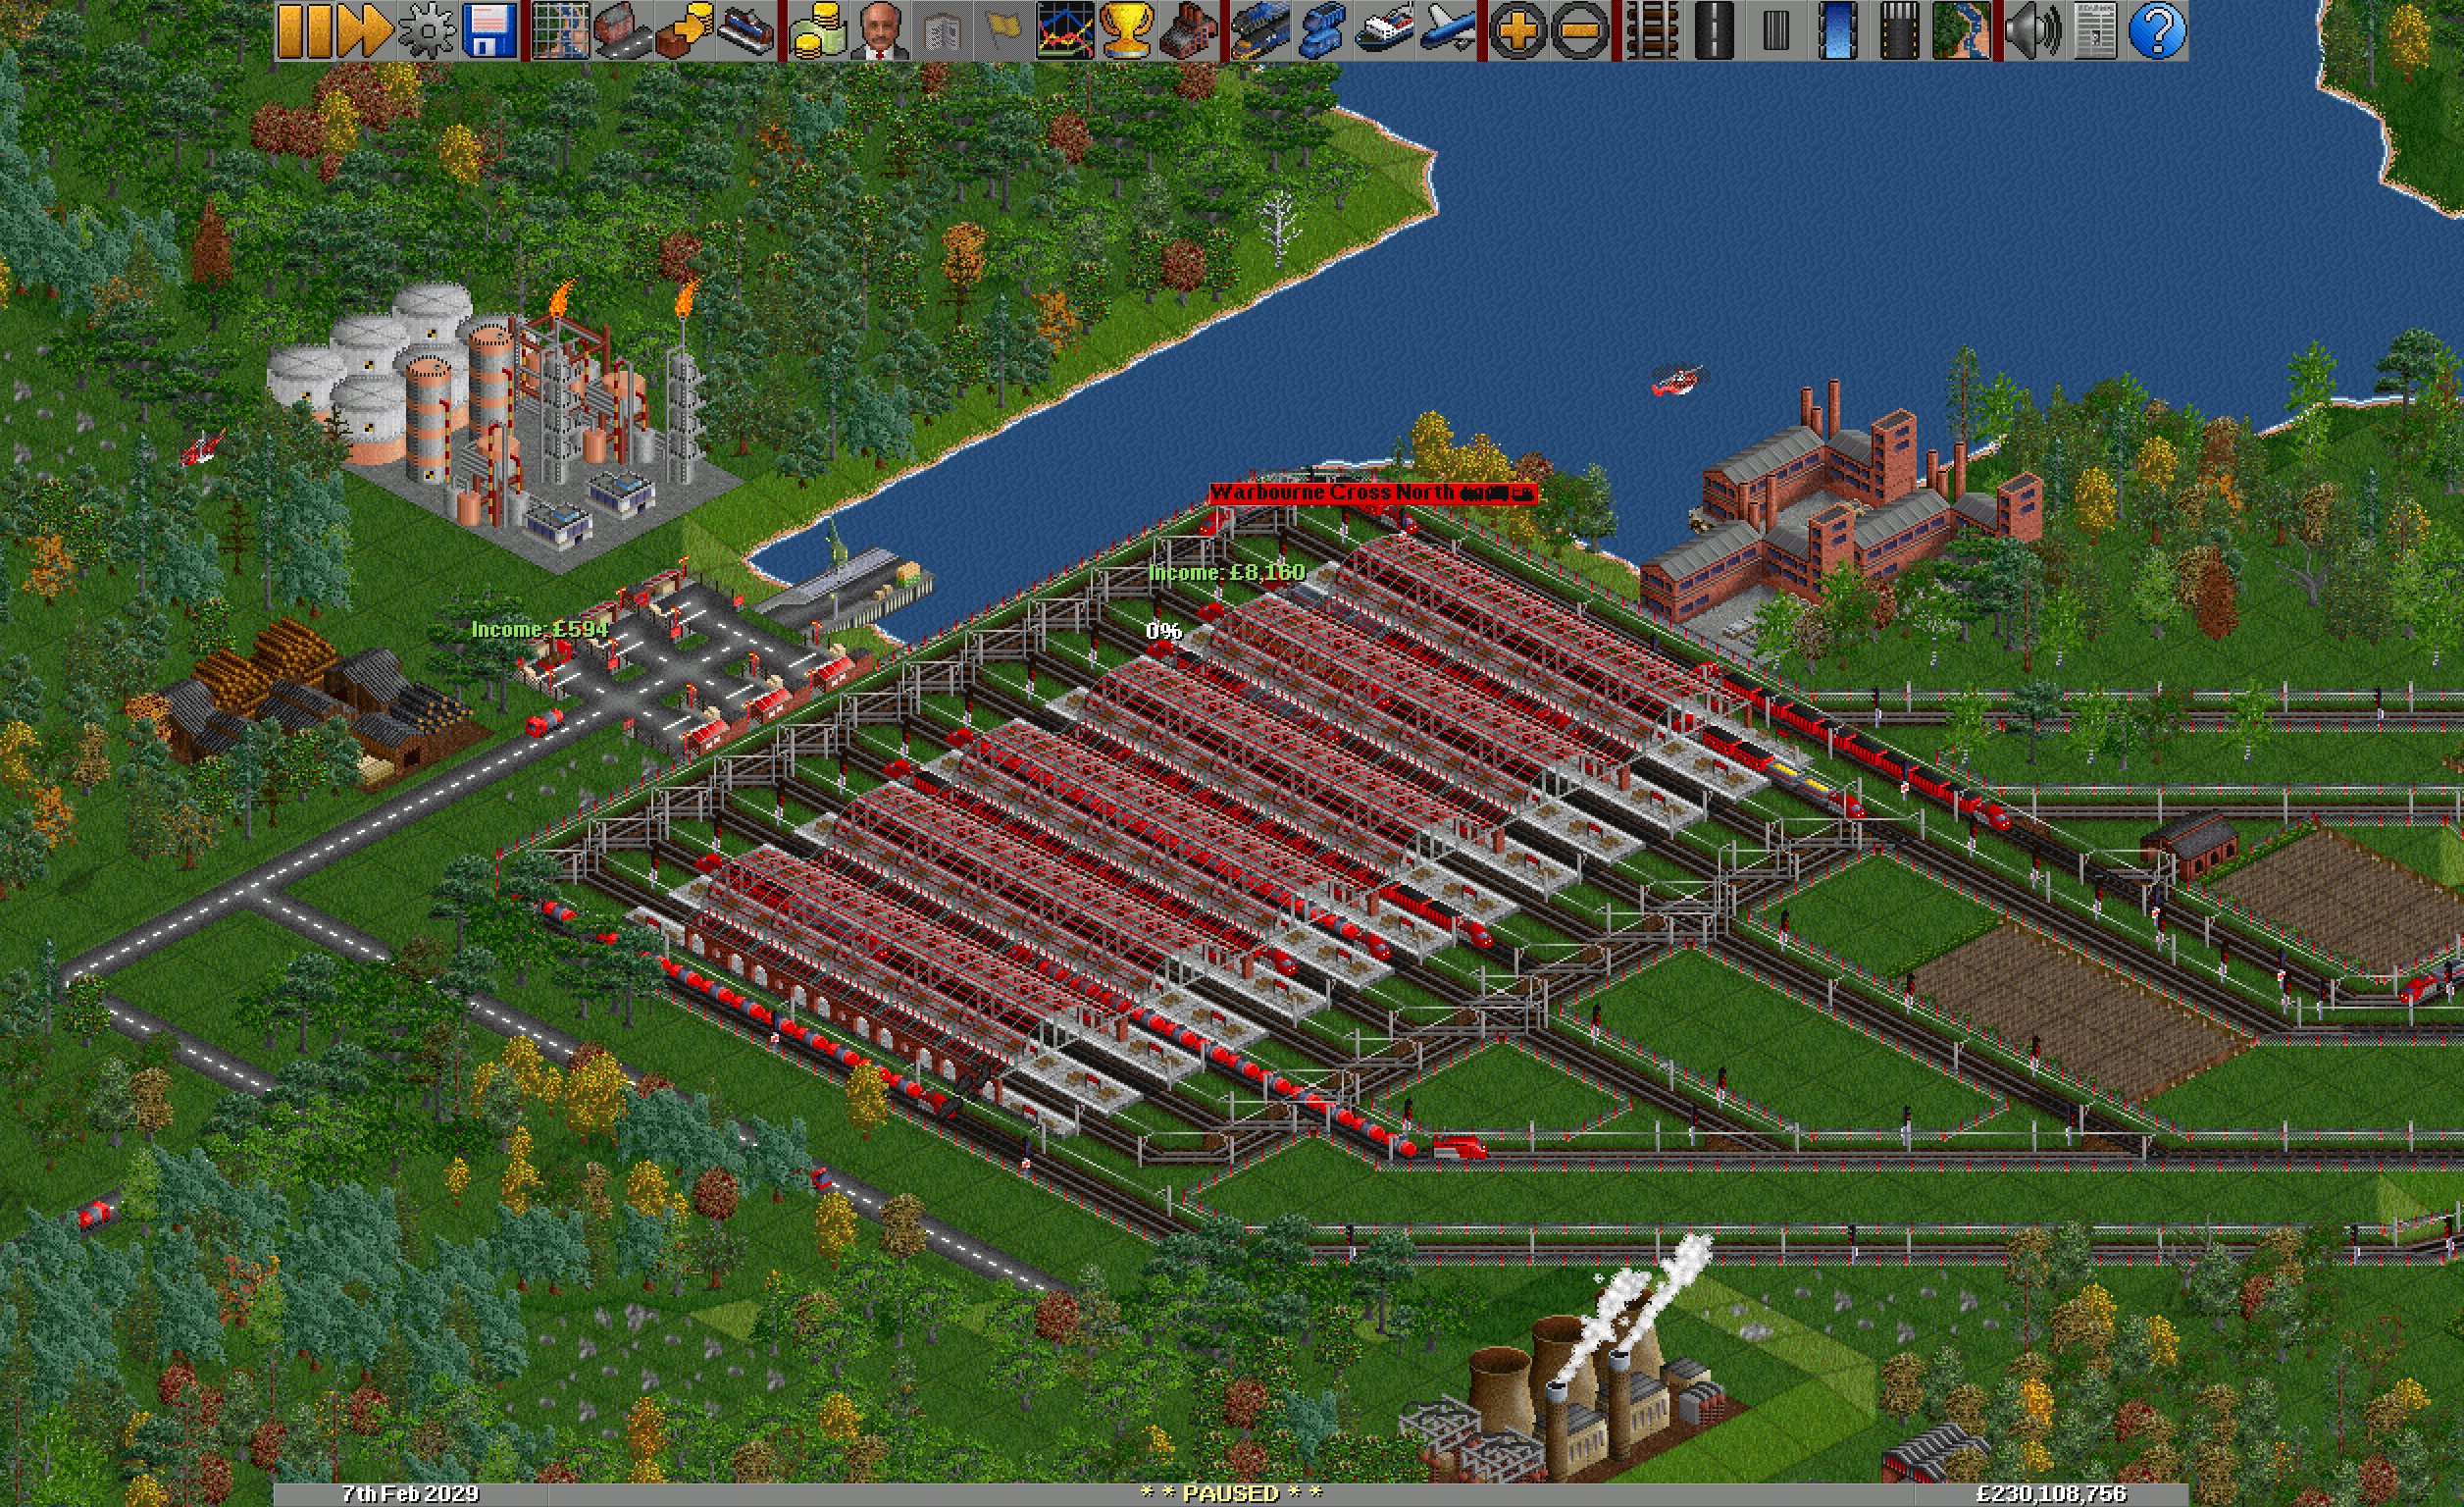
\includegraphics[width=\textwidth]{transport-tycoon-screenshot.png}
\caption{Screenshot of an OpenTTD game showing part of a transport network with multiple industries and mechanisms of transport. One of the trains has broken down, which not only prevents its cargo from reaching its destination, but it also prevents other trains from progressing along that track; OpenTTD has built-in ways of penalising non-robustness.}
\label{fig:network}
\end{figure}

OpenTTD is an open source business simulation game based on the 1990s game Transport Tycoon Deluxe. The aim of the game is to create a business that makes money from the transport of passengers and goods from one place to another, by constructing and using a network of road vehicles, trains, planes, or ships. An example of part of such a network can be seen in Figure \ref{fig:network}.

OpenTTD allows the implementation of so-called AIs, custom computer-based players that can compete with human players. Over 50 such AIs have been created. This project is to create and evaluate an AI that creates an AI that creates a network with good robustness properties. None of the 50 AIs have appear to focus on this aspect of the transport networks.

In the context of creation of goods, such networks are often referred to as supply chains. The study of supply chain robustness is an active area of research, especially into effects from the coronavirus (COVID-19) pandemic.

\subsection{Problem Statement}

The aim of this project is to create an OpenTTD AI that constructs networks that is robust to interruptions to parts of the transport network it constructs. Figure \ref{fig:network} shows an example of such an interruption - a broken down train that blocks its track. This analagous to real-world events such as the Ever Given blocking the Suez canel, distributing global supply chains for . No existing OpenTTD has been created or studied through this lens.

The evaluation of such networks. Potentially they could contribute to knowledge of real-world supply chains. For example, if the relationship between redundancy and robustness, these could lend w

OpenTTD allows the player to choose what business to focus on, or what method of travel to focus on.

\begin{itemize}
    \item Answer the question: ``What is the gap that needs to be filled?"
    and/or ``What is the problem that needs to be solved?"
    \item State the problem clearly early in a paragraph.
    \item Limit the variables you address in stating your problem.
    \item Consider bordering the problem as a question.
\end{itemize}

\subsection{Research Hypothesis and Objectives}

Identify the overall aims of the project and the individual measurable objectives against which you would wish the outcome of the work to be assessed. Clearly spell out any research hypothesis you are following.

Include a justification (rationale) for the study. Be clear about what your study will not address.

\subsection{Timeliness and Novelty}



Explain why the proposed research is of sufficient timeliness and novelty

\subsection{Significance}

The proposal should demonstrate the originality of your intended research. You should therefore explain why your research is important (for example, by explaining how your research builds on and adds to the current state of knowledge in the field or by setting out reasons why it is timely to research your proposed topic) and providing details of any immediate applications, including further research that might be done to build on your findings.

\subsection{Feasibility}

The existance of the 50 AIs suggests its not too

However, 

Comment on the feasibility of the research plans given its limited time frame and resources. Outline your plans for a feasibility study before starting eg major implementation work.

\subsection{Beneficiaries}

Describe how the research will benefit other researchers in the field and in related disciplines. What will be done to ensure that they can benefit? 


\section{Background and Related Work}

Demonstrate a knowledge and understanding of past and current work in the subject area, including relevant references like this \cite{template}.


\section{Programme and Methodology}

\begin{itemize}
    \item Detail the methodology to be used in pursuit of the research and justify this choice.
    \item Describe your contributions and novelty and where you
    will go beyond the state-of-the-art (new methods, new tools,
    new data, new insights, new proofs,\ldots)
    \item Describe the programme of work, indicating the research to be undertaken and the milestones that can be used to measure its progress.
    \item Where suitable define work packages and define the dependencies
    between these work packages. WPs and their dependencies should be
    shown in the Gantt chart in the research plan.
    \item Explain how the project will be managed.
    \item State the limitations of your research.
\end{itemize}

\subsection{Risk Assessment}



\subsection{Ethics}

All data will be generated during the project, and will not involve people.

\section{Evaluation}



\begin{itemize}
    \item Describe the specific methods of data collection.
    \item Explain how you intent to analyse and interpret the results.
\end{itemize}

\section{Expected Outcomes}

Conclude your research proposal by addressing your predicted outcomes. What are you hoping to prove/disprove? Indicate how you envisage your research will contribute to debates and discussions in your particular subject area:

\begin{itemize}
    \item How will your research make an original contribution to knowledge?
    \item How might it fill gaps in existing work? 
    \item How might it extend understanding of particular topics?
\end{itemize}


\section{Research Plan, Milestones and Deliverables}

\begin{figure}[htbp]
\begin{ganttchart}[
    vgrid,inline,
    x unit=1cm,
    time slot format=isodate-yearmonth,
    time slot unit=month,
    title height=1,
    group peaks height=0,
    group left shift=0,
    group right shift=0,
    group top shift=.7,
    bar height=.6
   ]{2023-05}{2024-08}
    \gantttitlecalendar{year, month=shortname} \\
    \ganttgroup{Prep}{2023-05}{2023-06} \\
    \ganttbar[name=dissertation, bar label font=\footnotesize]{Dissertation}{2023-05}{2023-06} \\
    \ganttbar[name=dissertation]{Compile}{2023-05}{2023-06} \\
    \ganttgroup{Headless mode}{2023-06}{2023-08} \\
    \ganttbar[name=i1]{1}{2023-06}{2023-06} \\
    \ganttbar[name=i2]{2}{2023-07}{2023-07} \ganttlink{i1}{i2} \\
    \ganttbar[name=i3]{3}{2023-08}{2023-08} \ganttlink{i2}{i3}  \\
    \ganttgroup{Basic AI}{2023-09}{2023-11} \\
    \ganttbar[name=i4]{4}{2023-09}{2023-09} \ganttlink[link mid=.25]{i3}{i4} \\
    \ganttbar[name=i5]{5}{2023-10}{2023-10} \ganttlink{i4}{i5}   \\
    \ganttbar[name=i6]{6}{2023-11}{2023-11} \ganttlink{i5}{i6}   \\  
    \ganttgroup{Robust AI}{2023-12}{2024-08} \\
    \ganttbar[name=i7]{7}{2023-12}{2023-12} \ganttlink[link mid=.25]{i6}{i7}  \\
    \ganttbar[name=i8]{8}{2024-01}{2024-01} \ganttlink{i7}{i8}  \\
    \ganttbar[name=i9]{9}{2024-02}{2024-02} \ganttlink{i8}{i9}  \\
    \ganttbar[name=i10]{10}{2024-03}{2024-03} \ganttlink{i9}{i10}  \\
    \ganttbar[name=i11]{11}{2024-04}{2024-04} \ganttlink{i10}{i11}  \\
    \ganttbar[name=i12]{12}{2024-05}{2024-05} \ganttlink{i11}{i12}  \\
    \ganttbar[name=i13]{13}{2024-06}{2024-06} \ganttlink{i12}{i13}  \\
    \ganttbar[name=i14]{14}{2024-07}{2024-07} \ganttlink{i13}{i14}  \\
    \ganttbar[name=i15]{15}{2024-08}{2024-08} \ganttlink{i14}{i15}  
\end{ganttchart}
\caption[Project Gantt chart]{Gantt Chart of the activities defined for this project. This project will be undertaken on a part time basis and in a highly iterative way. Each iteration will contain reading, development, evaluation, and writing up. Each will result in complete project, albeit with limited scope.}
\label{fig:gantt}
\end{figure}

\begin{table}[htbp]
    \begin{center}
        \begin{tabular}{|c|S[table-format=2.0]|l|}
        \hline
        \textbf{Milestone} & \textbf{Week} & \textbf{Description} \\
        \hline
        $M_1$ & 2 & Feasibility study completed \\
        $M_2$ & 5 & First prototype implementation completed \\
        $M_3$ & 7 & Evaluation completed \\
        $M_4$ & 10 & Submission of dissertation \\
        \hline
        \end{tabular} 
    \end{center}
    \caption[Project milestones]{Milestones defined in this project.}
    \label{fig:milestones}
\end{table}

\begin{table}[htbp]
    \begin{center}
        \begin{tabular}{|c|S[table-format=2.0]|l|}
        \hline
        \textbf{Deliverable} & \textbf{Week} & \textbf{Description} \\
        \hline
        $D_1$ & 6 & Headless mode for to OpenTTD \ldots\\
        $D_2$ & 8 & Evaluation report on \ldots\\
        $D_3$ & 10 & Dissertation \\
        \hline
        \end{tabular} 
    \end{center}
    \caption[Project deliverables]{List of deliverables defined in this project.}
    \label{fig:deliverables}
\end{table}


%                Now build the reference list
\bibliographystyle{unsrt}   % The reference style
%                This is plain and unsorted, so in the order
%                they appear in the document.

{\small
\bibliography{main}       % bib file(s).
}
\end{document}

